\documentclass{beamer} %[handout]
\usetheme{CambridgeUS}
\usecolortheme{whale}
\usepackage{color}
\usepackage{xcolor}
\usepackage[makeroom]{cancel}
\usepackage{graphicx} 
\setbeamercolor{frametitle}{fg=black}
\usepackage{mathtools}
\usepackage{amssymb}
\usepackage{amsmath}
\usepackage{amsthm}
\usepackage{graphicx}
\usepackage{fancyvrb}
\usepackage{listings}
\usepackage{tikz}
\usepackage[utf8]{inputenc}

\usetikzlibrary{shapes}

\usetikzlibrary{decorations.text}

\lstset{frame=tb,
  language=R,
  aboveskip=3mm,
  belowskip=3mm,
  showstringspaces=false,
  columns=flexible,
  basicstyle={\tiny\ttfamily},
  numbers=none,
  numberstyle=\tiny\color{gray},
%  keywordstyle=\color{blue},
%  identifierstyle=\color{yellow},
  breaklines=true,
    literate={->}{$\rightarrow$}{2}
           {°}{$\epsilon$}{1},
  breakatwhitespace=true
  tabsize=3
}

\usetikzlibrary{arrows,positioning} 
\tikzset{
    %Define standard arrow tip
    >=stealth',
    %Define style for boxes
    punkt/.style={
           rectangle,
           rounded corners,
           draw=black, very thick,
           text width=6.5em,
           minimum height=2em,
           text centered},
    % Define arrow style
    pil/.style={
           ->,
           thick,
           shorten <=2pt,
           shorten >=2pt,}
}

\makeatletter
\def\th@mystyle{%
    \normalfont % body font
    \setbeamercolor{block title example}{bg=orange,fg=white}
    \setbeamercolor{block body example}{bg=orange!20,fg=black}
    \def\inserttheoremblockenv{exampleblock}
  }
\makeatother
\theoremstyle{mystyle}
\newtheorem*{remark}{Example}

\makeatletter
\def\th@mystylet{%
    \normalfont % body font
    \setbeamercolor{block title example}{bg=purple,fg=white}
    \setbeamercolor{block body example}{bg=purple!20,fg=black}
    \def\inserttheoremblockenv{exampleblock}
  }
\makeatother
\theoremstyle{mystylet}
\newtheorem*{analysis}{Example}

\date{}
\author[Bayesian statistics]{Erik \v{S}trumbelj\\2019}

\linespread{1.2}
\renewcommand{\thefootnote}{\roman{footnote}}
%\setbeameroption{show notes}

\title[Linear regression]{Linear regression}

\begin{document}

\begin{frame}

\begin{center}
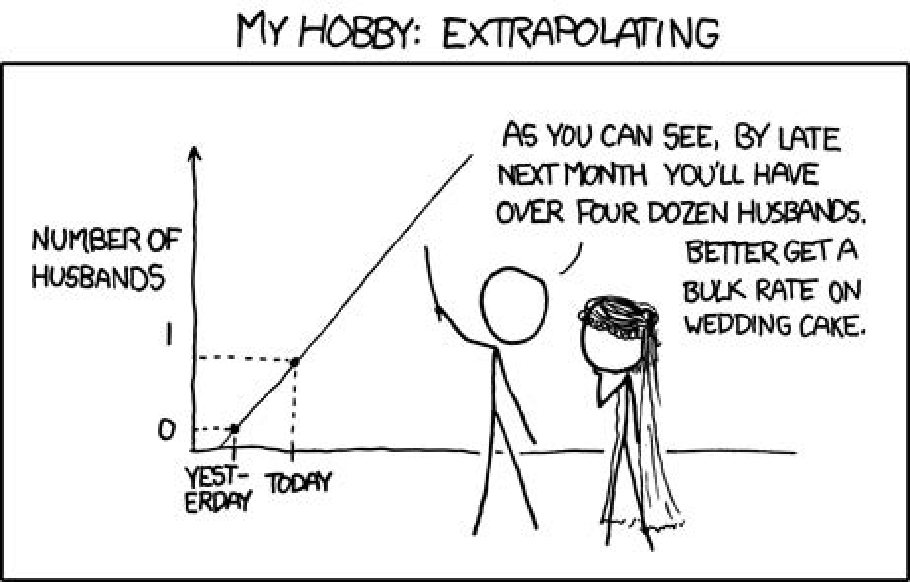
\includegraphics[width=0.90\linewidth]{../LectureAssets/L04/Lecture04cartoon}
\end{center}

\end{frame}

\begin{frame}
Bayesian statistics
\titlepage
\end{frame}

\begin{frame}
\begin{analysis}[Simple bivariate distribution]
\smallskip
200 samples of (x,y) pairs:
\smallskip
\begin{center}
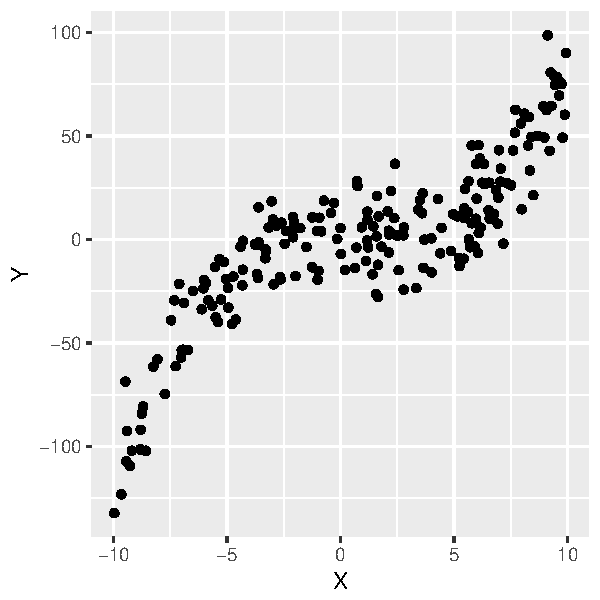
\includegraphics[width=0.40\linewidth]{../LectureAssets/L04/SimpleReg01}
\end{center}
\smallskip
We wish to model the relationship between $x$ and $y$, with the purpose of predicting $y$ for future observations of $x$.
\smallskip
\end{analysis}
\end{frame}

\begin{frame}
\begin{analysis}[Modelling with a line]

\smallskip

There are infinitely many lines:

\bigskip
\begin{center}
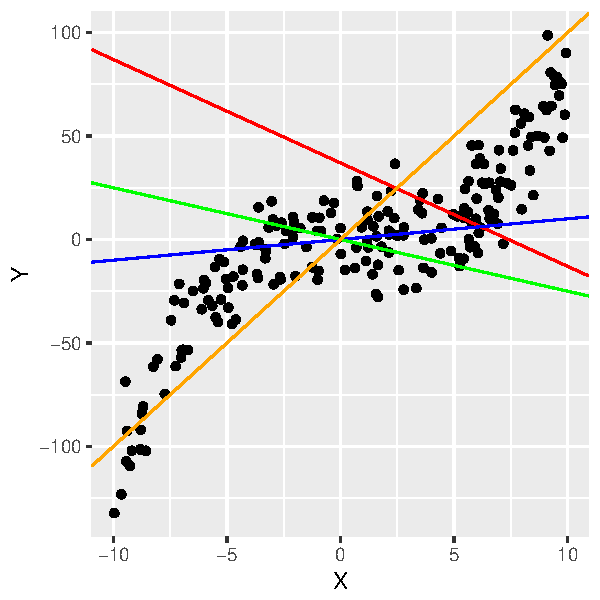
\includegraphics[width=0.40\linewidth]{../LectureAssets/L04/SimpleReg02}
\end{center}

\smallskip

No line gives a perfect fit. Which one is the best?

\smallskip
\end{analysis}
\end{frame}


\begin{frame}{Simple linear model}

Model:

\bigskip

$ y_i = \beta_2 x_{i} + \beta_1 + \epsilon_i, \text{   }$\hfill$\epsilon \sim_\text{iid} \mathcal{N}(0, \sigma^2), i = 1..n$.

\bigskip

Or, equivalently:

\bigskip

$$y_i \sim \mathcal{N}(\beta_2 x_{i} + \beta_1, \sigma^2).$$

\bigskip

Selecting the line that maximizes the likelihood:

$$p( y |  x, \beta_1, \beta_2, \sigma^2) = \prod_{i=1}^n \frac{1}{\sqrt{2\pi\sigma^2}} e^{-\frac{(y_i - \beta_2 x_{i} - \beta_1)^2}{2\sigma^2}}$$

\end{frame}

\begin{frame}
\begin{analysis}[Simple linear model]

\smallskip

Maximum likelihood estimates: $\beta_2 = 5.96, \beta_1 = -5.49, \sigma = 21.65$:

\bigskip
\begin{center}
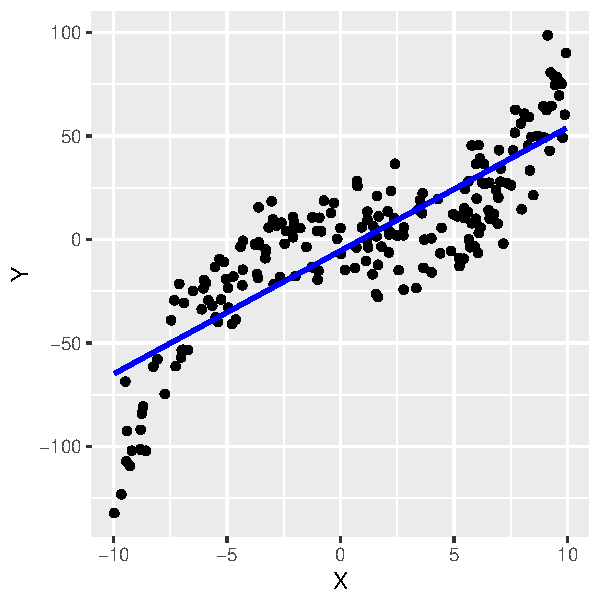
\includegraphics[width=0.40\linewidth]{../LectureAssets/L04/SimpleReg03}
\end{center}

\smallskip

\smallskip
\end{analysis}
\end{frame}


\begin{frame}{Linear regression}

Simple generalization to $k$:

\bigskip

$ y_i = \beta_k x_{i,k} + ... + \beta_2 x_{i,2} + \beta_1 x_{i,1} + \epsilon_i, \text{   }$\hfill$\epsilon \sim_\text{iid} \mathcal{N}(0, \sigma^2), i = 1..n$.

\bigskip

Or, equivalently:

\bigskip

$y_i \sim \mathcal{N}(   \beta^T  x_i, \sigma^2)$ or $ y \sim \mathcal{N}_n( X \beta , \sigma^2\mathbb{I})$.

\bigskip

The likelihood
\begin{scriptsize}
$$p( y |  X,  \beta, \sigma^2)  = \left(\frac{1}{\sqrt{2\pi\sigma^2}}\right)^n e^{-\frac{\sum_{i=1}^n (y_i -  \beta^T  x_{i})^2}{2\sigma^2}}  = \left(\frac{1}{\sqrt{2\pi\sigma^2}}\right)^n e^{-\frac{SSR( \beta)}{2\sigma^2}}.$$
\end{scriptsize}

is maximized by $ \beta^* = ( X^T  X)^{-1}  X^T  y $ (Ordinar Least Squares).

\end{frame}


\begin{frame}
\begin{analysis}[Bayesian linear regression]

\smallskip

Gibbs sampling (m = 5000; $ \beta_0 =  0, \Sigma_0 = 2500\mathbb{I},a_0 = 1$, $b_0 = 20$):

\bigskip

\begin{minipage}[c]{0.47\linewidth}
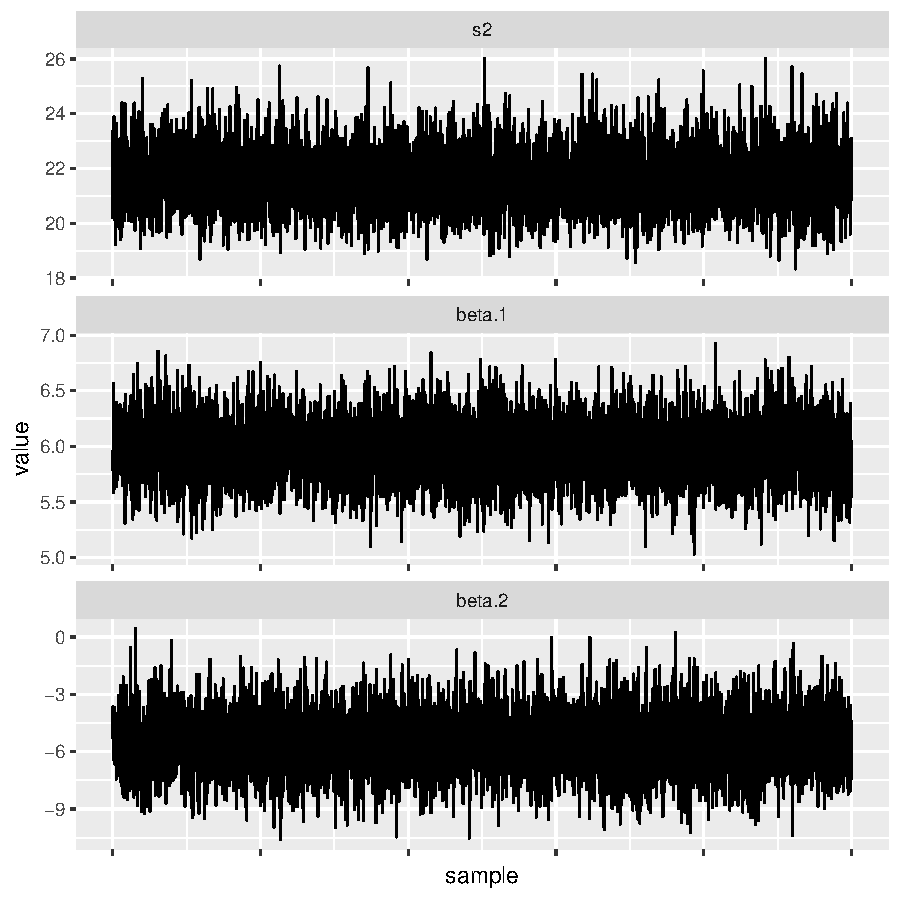
\includegraphics[width=0.9\linewidth]{../LectureAssets/L04/SimpleReg04}
\end{minipage} 
\begin{minipage}[c]{0.47\linewidth}
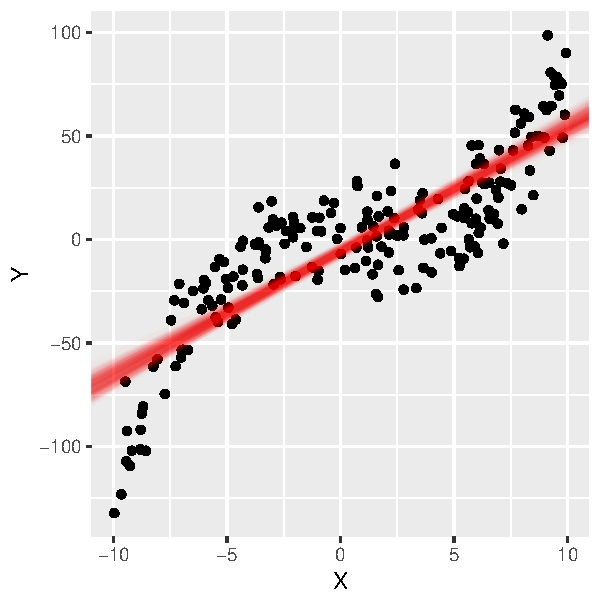
\includegraphics[width=0.9\linewidth]{../LectureAssets/L04/SimpleReg05}
\end{minipage} 

\smallskip

All $m_{eff} > 4000$, $se_{MCMC} < 0.05$.

\smallskip

\begin{tiny}
Bayesian posterior means: \hfill $\beta_1 = 5.96, \beta_0 = -5.49, \sigma = 21.63$

Maximum likelihood estimates: \hfill $\beta_1 = 5.96, \beta_0 = -5.49, \sigma = 21.65$
\end{tiny}

\smallskip
\end{analysis}
\end{frame}

\begin{frame}
\begin{analysis}[Simple linear regression]

\bigskip

\bigskip

\smallskip

\begin{center}
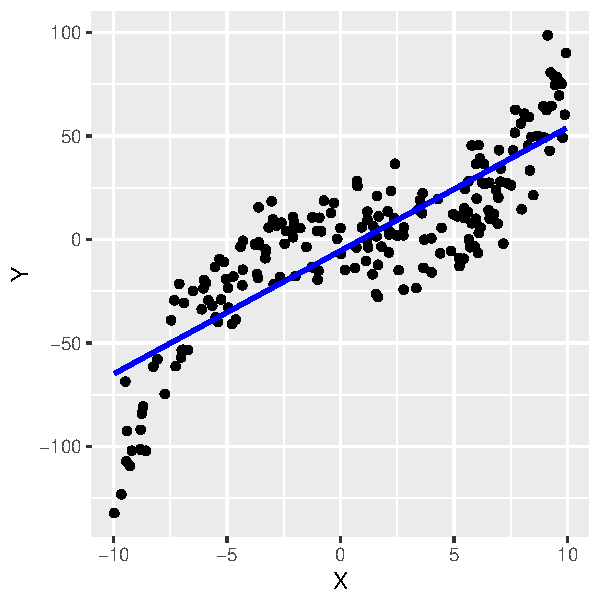
\includegraphics[width=0.40\linewidth]{../LectureAssets/L04/SimpleReg03}
\end{center}

Any suggestions for a more appropriate model?

\smallskip
\end{analysis}
\end{frame}

\begin{frame}
\begin{analysis}[Non-linearity via input space transformation]

\bigskip

This is still linear regression:
$$ y_i = \beta_k x^k_{i} + ... + \beta_2 x^2_{i} + \beta_1 x_{i}  + \beta_0 + \epsilon_i$$

\smallskip

\bigskip

\begin{minipage}[c]{0.24\linewidth}
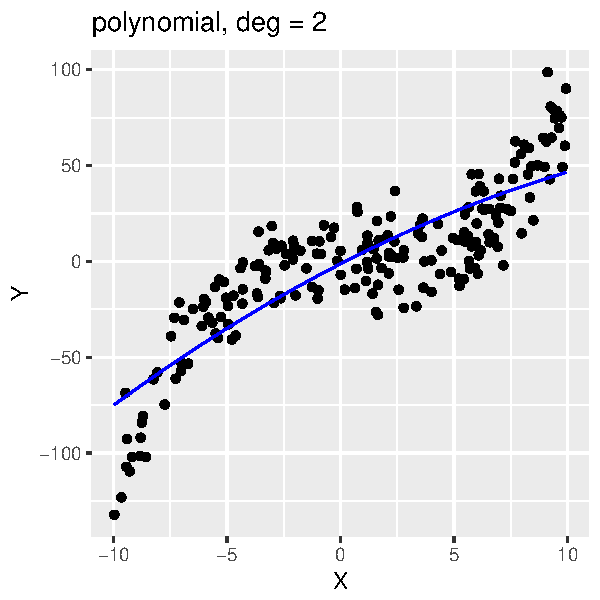
\includegraphics[width=1.0\linewidth]{../LectureAssets/L04/SimpleRegCV2}
\end{minipage} 
\begin{minipage}[c]{0.24\linewidth}
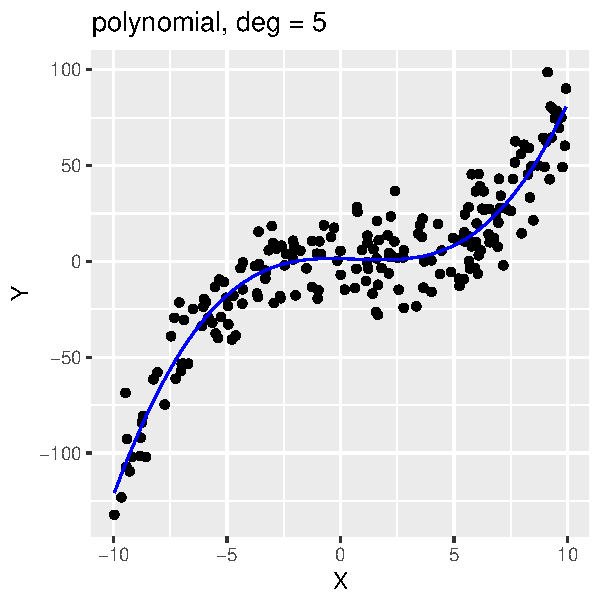
\includegraphics[width=1.0\linewidth]{../LectureAssets/L04/SimpleRegCV5}
\end{minipage} 
\begin{minipage}[c]{0.24\linewidth}
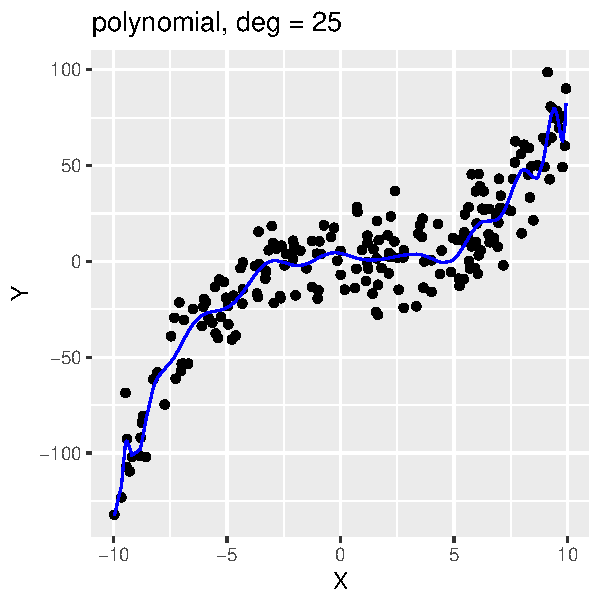
\includegraphics[width=1.0\linewidth]{../LectureAssets/L04/SimpleRegCV25}
\end{minipage} 
\begin{minipage}[c]{0.24\linewidth}
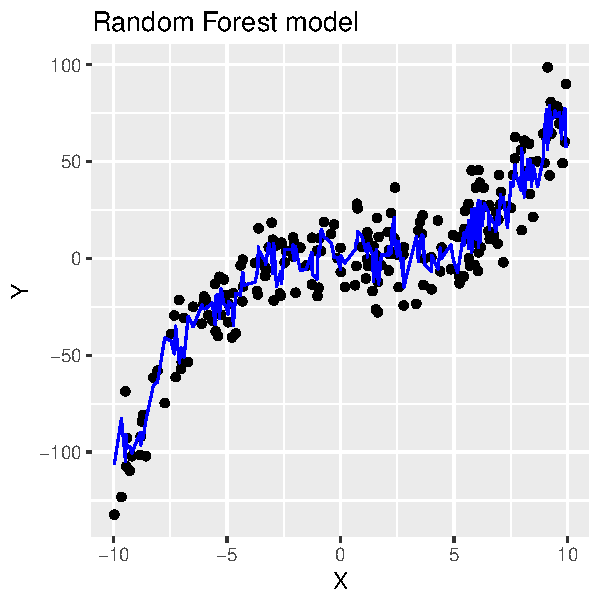
\includegraphics[width=1.0\linewidth]{../LectureAssets/L04/SimpleRegCVRF}
\end{minipage} 


\bigskip

\textbf{Which model is the best?}

\bigskip

\bigskip

\end{analysis}
\end{frame}

\begin{frame}{Model selection}

\begin{Large}

\bigskip

The goal is to select a model that will best generalize to new (unseen) data from the problem.

\bigskip

Two key components:

\begin{itemize}
\item Error (quality) criterion.
\item Error estimation procedure.
\end{itemize}
\end{Large}

\bigskip

\end{frame}

\begin{frame}{Error criteria}

In general, the log-score (log-likelihood) is a good choice:

$$LOG = \log \left(\overbrace{\prod_{i=1}^n p_{model}(y_i|y)}^{\text{likelihood}}\right) = \sum_{i=1}^n \log p_{model}(y_i|y).$$

\bigskip

Often, especially in machine learning, Mean Squared Error (MSE) is used:

$$MSE = \frac{1}{n} \sum_{i=1}^n (y_{\text{model}} - y_i)^2.$$

\bigskip

\bigskip

Other: accuracy, precision, recall, rank probability score, Brier score,...

\end{frame}

\begin{frame}{Procedure for error estimation}

Estimating error on the dataset used for fitting the model will result in biased (optimistic) estimates.

\bigskip

\textbf{Alternative 1 (separate evaluation dataset):} Reserve a random subset for evaluation and use the rest for fitting the model.

\bigskip

\textbf{Alternative 2 (cross-validation):} 

\bigskip

\begin{itemize}
\item Partition the data into $k$ (approximately) equal parts: $ y_1$, $ y_2$, ..., $ y_k$.
\item Fit $k$ models $M_i, i = 1..k$, each without the $i$-th partition.
\item Estimate error with $\overline{err} \approx \frac{1}{n} \sum_{i=1}^k  \sum_{j=1}^{n_i} err_{M_i}(y_{i,j})$.
\end{itemize}

\bigskip

Special case $k = n$: leave-one-out cross-validation (LOOCV).
\end{frame}

\begin{frame}
\begin{analysis}[Model evaluation]


\begin{minipage}[c]{0.24\linewidth}
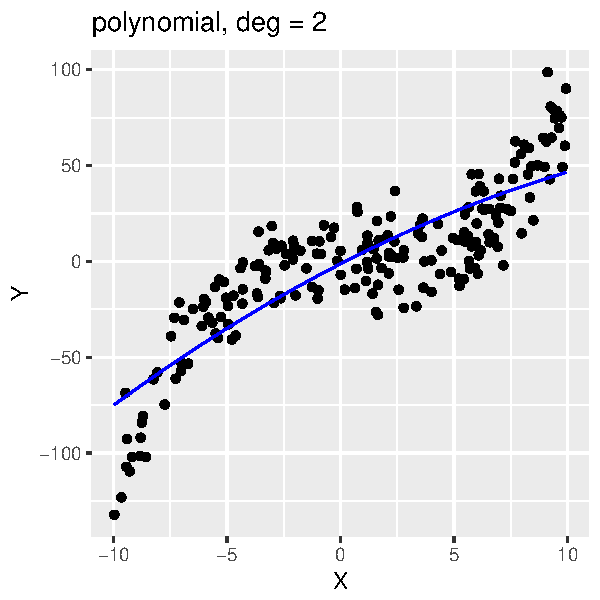
\includegraphics[width=1.0\linewidth]{../LectureAssets/L04/SimpleRegCV2}
\end{minipage} 
\begin{minipage}[c]{0.24\linewidth}
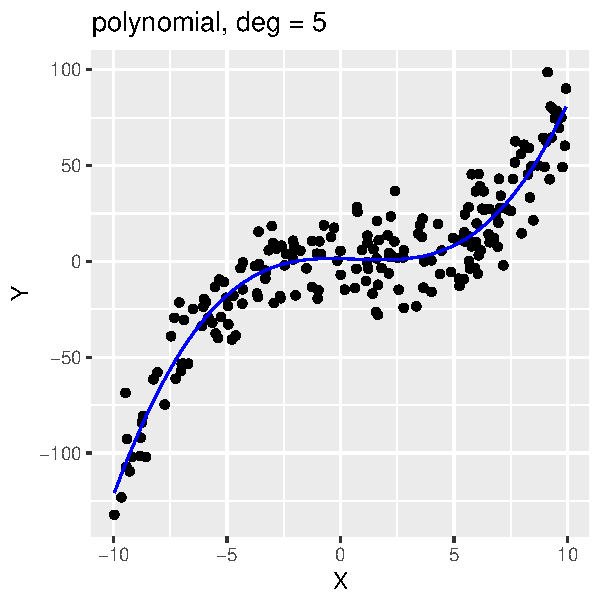
\includegraphics[width=1.0\linewidth]{../LectureAssets/L04/SimpleRegCV5}
\end{minipage} 
\begin{minipage}[c]{0.24\linewidth}
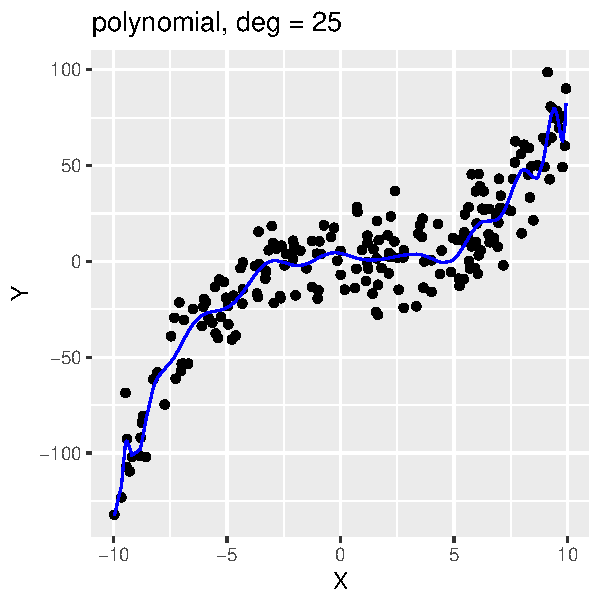
\includegraphics[width=1.0\linewidth]{../LectureAssets/L04/SimpleRegCV25}
\end{minipage} 
\begin{minipage}[c]{0.24\linewidth}
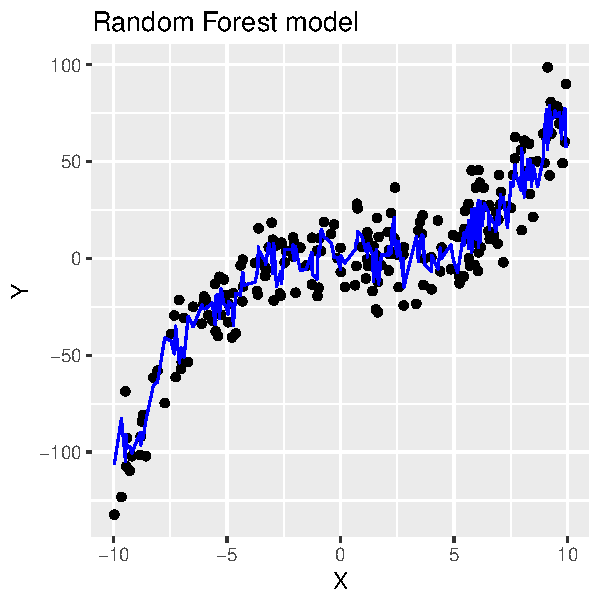
\includegraphics[width=1.0\linewidth]{../LectureAssets/L04/SimpleRegCVRF}
\end{minipage} 
\bigskip

In-sample and out-of-sample estimated (LOOCV) MSE:

\begin{scriptsize}
\begin{center}
\begin{tabular}{lcc}
\hline
Model & in-sample & out-of-sample \\
\hline
linear &464.1  & 475.8\\
2nd &450.0   &468.7\\
3rd &200.1   &208.6\\
5th &199.8   &213.1\\
25th &180.5 &12859.4\\
RF   &299.1 &296.9 \\
\hline
\hline
\end{tabular}
\end{center}
\end{scriptsize}

\smallskip

\end{analysis}
\end{frame}


\begin{frame}{Overfitting}

Fitting to the noise in the data and not the data generating process.

\bigskip

Consequence: incorrect inference, poor generalization and predictions for new/unseen data.

\bigskip

A proper procedure of estimating the models error will detect overfitting and there exist several approaches to preventing overfitting:

\begin{itemize}
\item feature selection,
\item early stopping,
\item tree pruning,
\item \textbf{regularization},
\item ...
\end{itemize}

\end{frame}

\begin{frame}
\begin{analysis}[Bear weight]

\smallskip

\begin{minipage}[c]{0.33\linewidth}
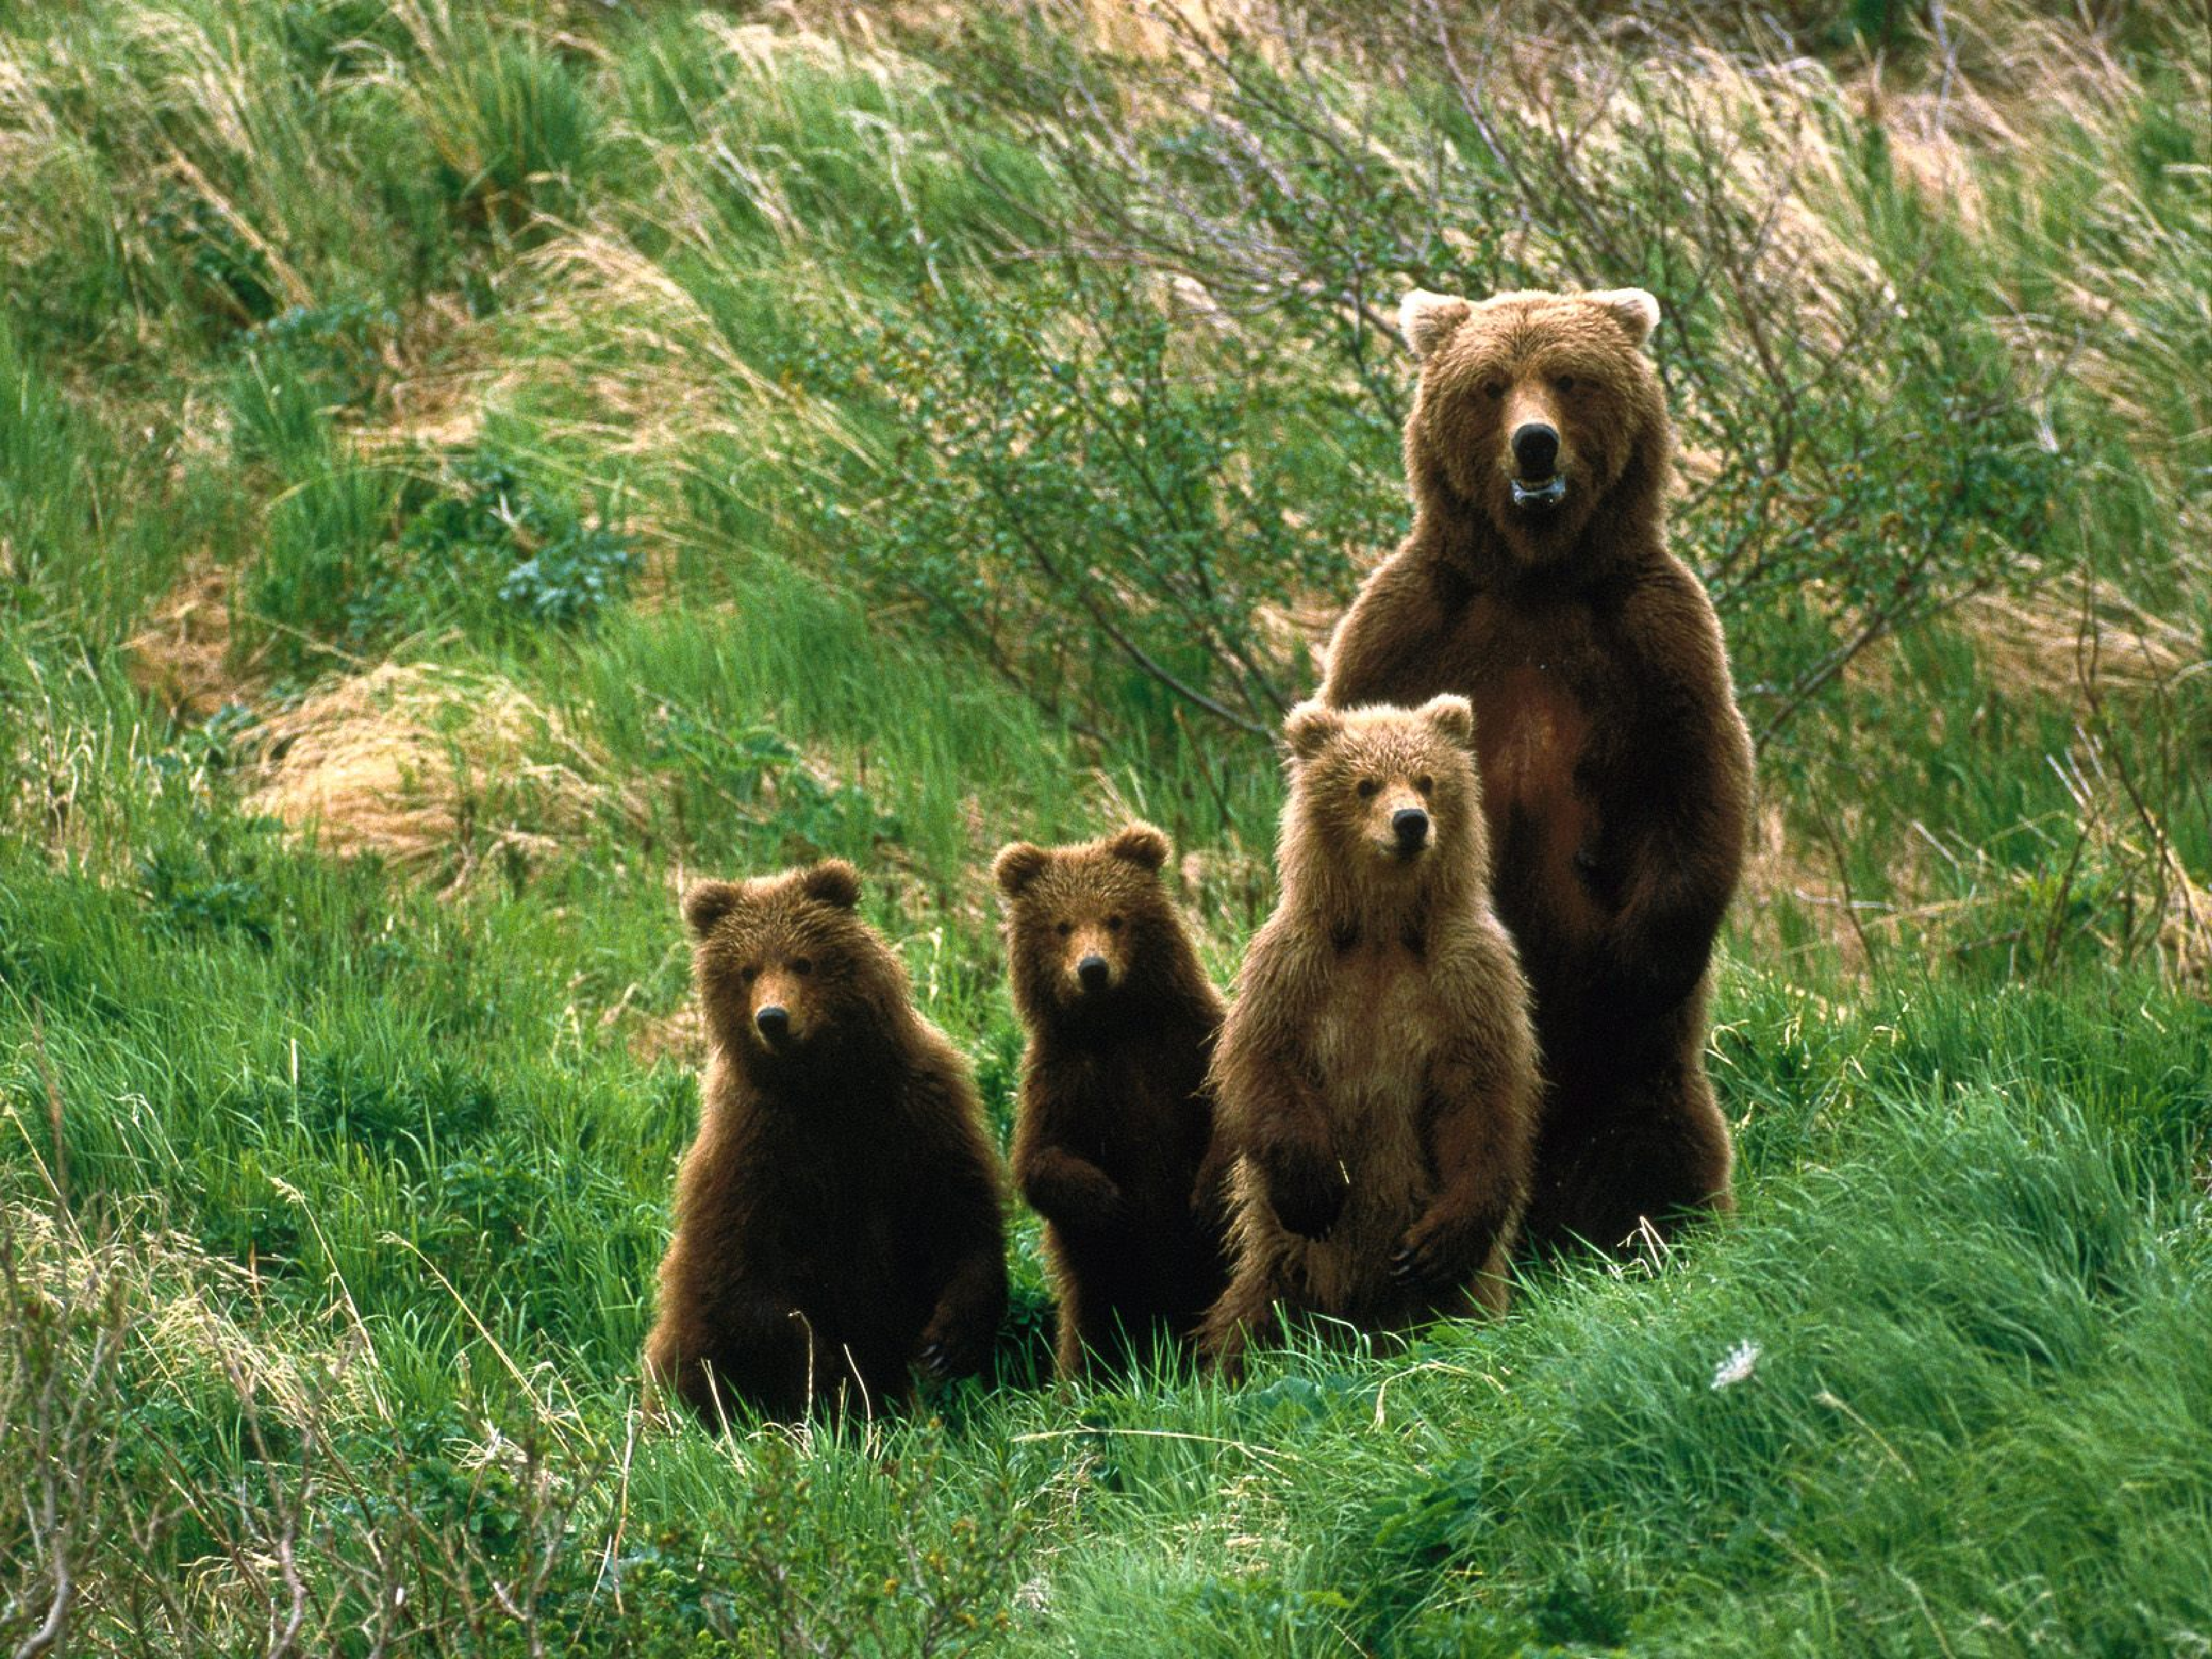
\includegraphics[width=1.0\linewidth]{../LectureAssets/L04/bear}
\end{minipage} 
\begin{minipage}[r]{0.65\linewidth}
\begin{tiny}
\tabcolsep=0.11cm
\hfill\begin{tabular}{cccccccc}
\hline
AGE	&  SEX & HEAD$_L$	& HEAD$_W$	& NECK	& LENGTH	& CHEST & \textbf{WEIGHT} \\
\hline
19	&  1	&11	  & 5.5	&16  &53    &26	& 80 \\
55	&  1	&16.5 &	9	&28  &67.5	&45 &	344\\
81	&  1	&15.5 &	8	&31	 &72	&54	&416\\
115	&  1	&17	  & 10	&31.5&72	&49 &	348\\
104	&  2	&15.5 &	6.5	&22	 &62	&35	&166\\
100	&  2	&13   &	7   &21	 &70	&41	&220\\
56	&  1 &	15&	7.5 &26.5&73.5  &41 &262\\
... \\
\hline
\hline
\end{tabular}
\end{tiny}
\end{minipage}

\bigskip

Random sample of 54 bears. 

\bigskip

Task:

\begin{itemize}
\item Predict bear weight from other variables: .
\end{itemize}

\bigskip

\end{analysis}
\end{frame}

\end{document}
